\section{Pianificazione}
	Il gruppo \cod\ ha scelto di utilizzare il \textbf{modello incrementale} come modello di sviluppo per la produzione del software \hd .
	Alla luce delle scadenze riportate nella sezione 1.5 e alle scadenze interne si è deciso di dividere il progetto in cinque fasi:
	\begin{itemize}
		\item \textbf{Analisi};
		\item \textbf{Consolidamento dei requisiti};
		\item \textbf{Progettazione architetturale};
		\item \textbf{Progettazione di dettaglio e codifica};
		\item \textbf{Validazione e collaudo}.
	\end{itemize}
	Ognuna di queste cinque fasi sarà formata da diverse sotto attività mostrate nel corrispettivo diagramma di Gantt.

	\subsection{Analisi}	\textbf{Periodo}: dal 26-11-2020 al 10-01-2021 \\
	La fase di Analisi è composta da sei attività che corrispondono alla produzione dei relativi documenti:
	\begin{itemize}
		\item \textbf{Studio di fattibilità}: ogni capitolato proposto viene analizzato e discusso con i membri del gruppo. Ogni capitolato viene poi classificato in base alle preferenze e ai punti di interesse riscontrati. Il capitolato che avrà riscosso più preferenze viene scelto come capitolato effettivo;
		\item \textbf{Norme di progetto}: vengono definite le regole che il team dovrà rispettare durante lo sviluppo del progetto;
		\item \textbf{Piano di Progetto}: si analizzato le attività, i compiti e le risorse che verranno distribuite tra i membri del team, presenta il calcolo del preventivo per la realizzazione del progetto;
		\item \textbf{Analisi dei requisiti}: vengono studiati e analizzati i requisiti del capitolato scelto nello studio di fattibilità;
		\item \textbf{Piano di qualifica}: durante questa attività si individuano le metodologie da usare per garantire la qualità del prodotto;
		\item \textbf{Glossario}: Questo documento viene redatto per definire la terminologia usata al fine di evitare ambiguità.
	\end{itemize}
	\subsubsection{Diagramma}
		\begin{figure}[H]
        		\centering
        		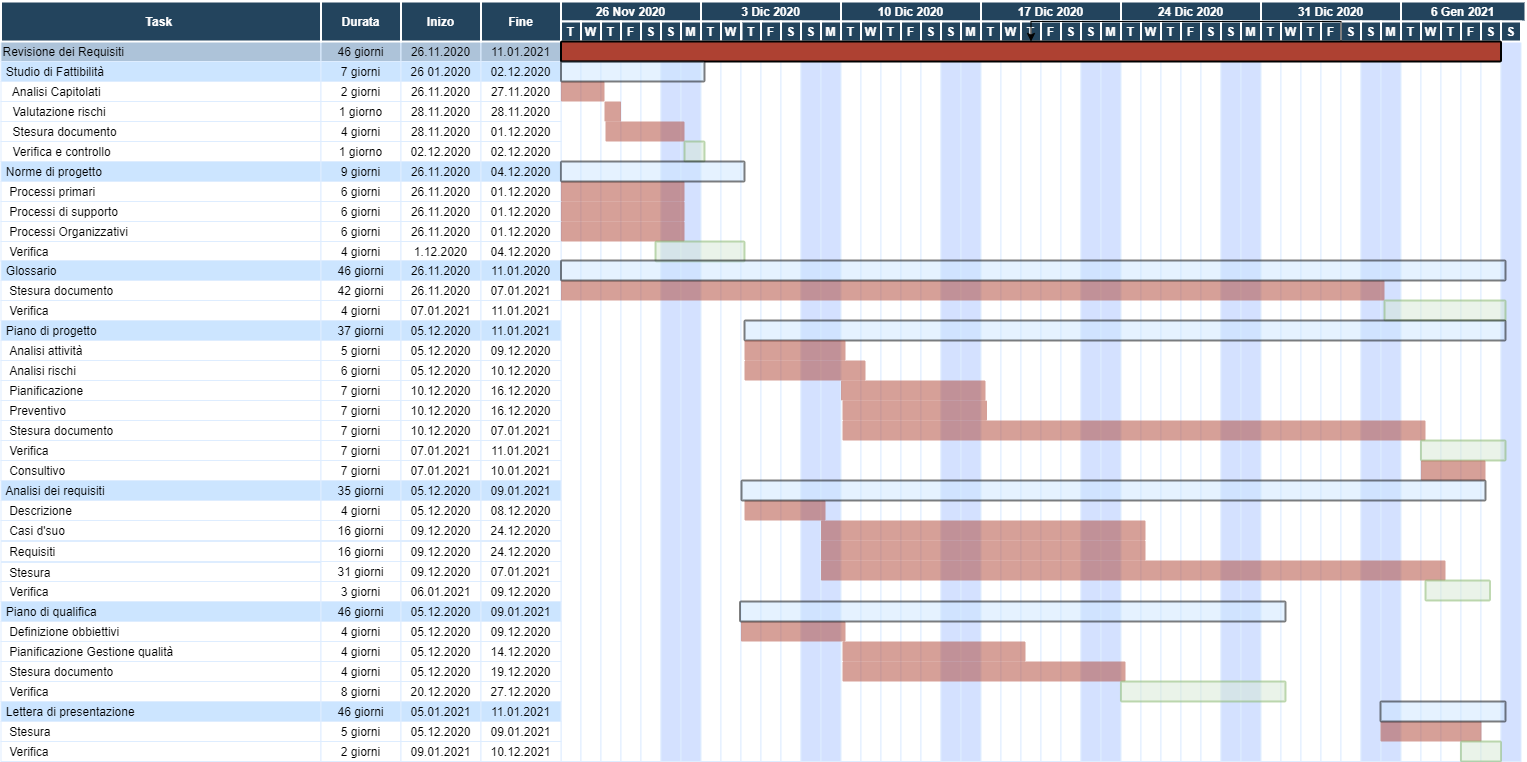
\includegraphics[width=\textwidth]{source/img/analisiattivita.png}
        		\caption{Diagramma di Gantt dell'attività di analisi}
    		\end{figure}

	\subsection{Consolidamento dei requisiti}
	\textbf{Periodo}: dal 12-01-2021 al 18-01-2021 \\
	La fase di consolidamento dei requisiti è intermedia tra la fine dell'attività di Analisi e il giorno della presentazione della Revisione dei Requisiti. \\
	Durante la seguente fase si svolgeranno attività di consolidamento dei requisiti osservati nella fase precedente e verrà preparata la presentazione per la Revisione dei Requisiti.
	
	\subsubsection{Diagramma}
		\begin{figure}[H]
        		\centering
        		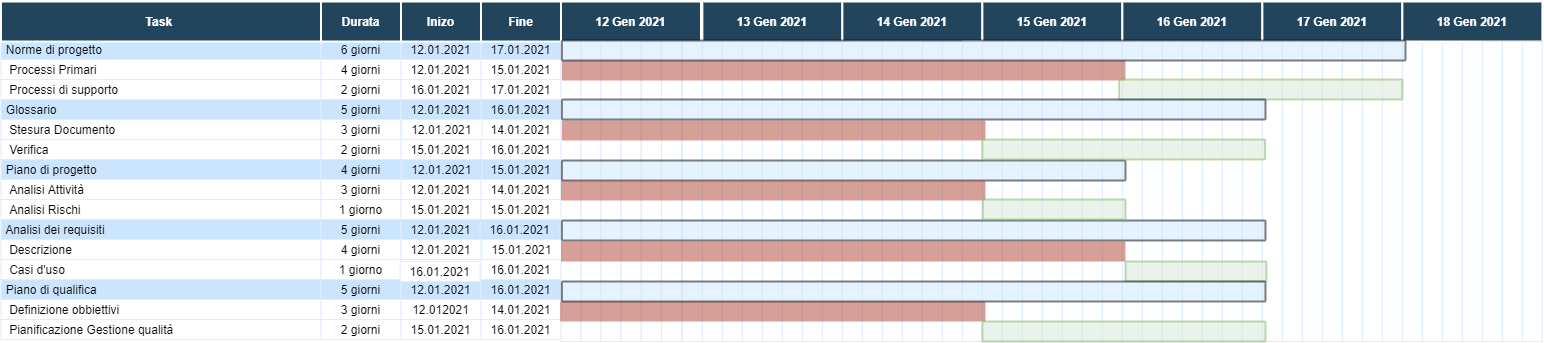
\includegraphics[width=\textwidth]{source/img/Consolidamento_Requisiti.png}
        		\caption{Diagramma di Gantt dell'attività di consolidamento requisiti}
    		\end{figure}
	
	\subsection{Progettazione architetturale}
	\textbf{Periodo}: dal 19-01-2021 al 01-03-2021 \\
	Successivamente alla presentazione della Revisione dei Requisiti inizia la fase di progettazione architetturale che terminerà con la consegna della Revisione di Progettazione, lo scopo di questo periodo è l'individuazione di una soluzione architetturale che soddisfi i seguenti requisiti:
	\begin{itemize}
		\item \textbf{Technology Baseline}: verrà stilato l'allegato tecnico nel quale verranno individuati i design pattern che verranno adottati nello sviluppo del progetto. Inoltre verrà redatto il Proof Of Concept da consegnare al committente;
		\item \textbf{Incremento di controllo}: se necessario vengono migliorati i documenti consegnati durante la fase iniziale;
		\item \textbf{Incremento di sviluppo}: i documenti prodotti saranno aggiornati per rispecchiare l'attuale andamento del progetto.
	\end{itemize}
	
	\subsubsection{Diagramma}
		\begin{figure}[H]
        		\centering
        		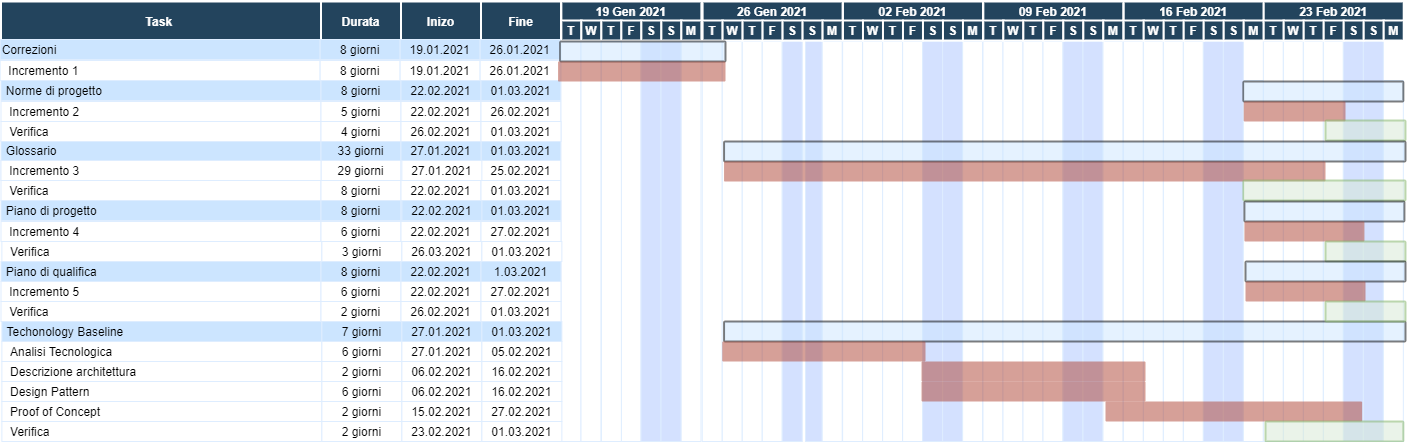
\includegraphics[width=\textwidth]{source/img/Progettazione_architetturale.png}
        		\caption{Diagramma di Gantt dell'attività di progettazione architetturale}
    		\end{figure}
	\subsubsection{Tabella incrementi}
		\begin{center}
    			\begin{tabular}{ | l | p{5cm} | p{8cm} |}
   			 \hline
    			Nome & Periodo & Descrizione \\ \hline
    			Incremento 1 & 19-01-2021 al 26-01-2021 & Ricevuto il feedback del committente i prodotti verranno aggiornati per risolvere le problematiche riscontrate. \\ \hline
    			Incremento 2 & 22-02-2021 al 01-03-2021 & Il documento Norme di Progetto verrà aggiornato per rispecchiare l'attuale situazione del progetto \\ \hline
    			Incremento 3 & 22-02-2021 al 01-03-2021 & Il documento Glossario verrà aggiornato per rispecchiare l'attuale situazione del progetto \\ \hline
			Incremento 4 & 22-02-2021 al 01-03-2021 & Il documento Piano di progetto verrà aggiornato per rispecchiare l'attuale situazione del progetto \\ \hline
			Incremento 5 & 22-02-2021 al 01-03-2021 & Il documento Piano di qualifica verrà aggiornato per rispecchiare l'attuale situazione del progetto \\ \hline
    			\end{tabular}
		\end{center}
	
	\subsection{Progettazione di dettaglio e codifica}
	\textbf{Periodo}: dal 11-03-2021 al 5-04-2021 \\
	Col termine della Revisione di Progettazione, inizia la fase di progettazione di dettaglio e codifica e terminerà con la Revisione di Qualifica, la seguente fase coinvolge i seguenti nuovi prodotti:
	\begin{itemize}
		\item \textbf{Product Baseline}: vengono studiati i design pattern, classi e attività necessarie alla codifica;
		\item \textbf{Manuale dello sviluppatore}: dentro il quale confluisce il materiale preparato per la Product Baseline;
		\item \textbf{Manuale Utente}: redazione del manuale utente del prodotto.
	\end{itemize}
	
	\subsubsection{Diagramma}
		\begin{figure}[H]
        		\centering
        		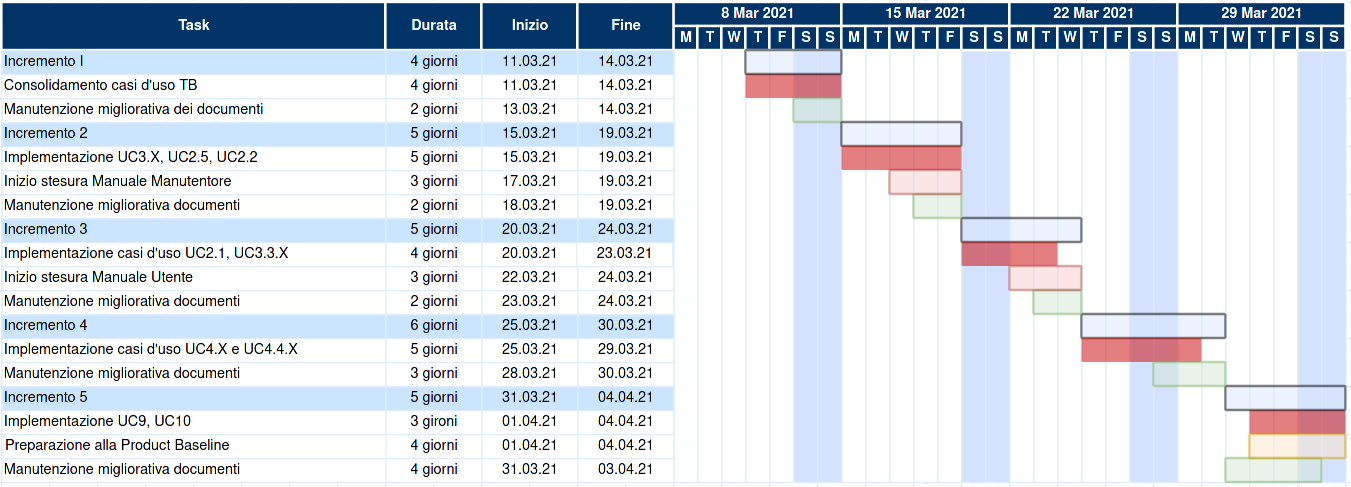
\includegraphics[width=\textwidth]{source/img/Progettazionedettaglio_codifica.png}
        		\caption{Diagramma di Gantt dell'attività di progettazione di dettaglio e codifica}
    		\end{figure}
	\subsubsection{Tabella incrementi}
    		\begin{longtabu} to \textwidth{| X[0.2, c m] | X[0.4, l m ] |}
   				\hline
					 \textbf{Nome} & \textbf{Descrizione} \\ 
					\hline
						\multicolumn{2}{|c|}{\textbf{Incremento 1}} \\
					\hline
						Consolidamento dei casi d'uso TB &
						Per il POC sono stati realizzati i seguenti casi d'uso: UC1.X, UC2.4, UC6.X. Sarà verificato e migliorato il codice. \\
					\hline
						Manutenzione migliorativa dei documenti &
						In particolare: saranno creati i test di integrazione all'interno dell'apposita sezione del Piano di Qualifica. \\
					\hline
						\multicolumn{2}{|c|}{\textbf{Incremento 2}} \\
					\hline
						Implementazione UC3.X, UC2.5, UC2.2 &
						Implementazione dei casi d'uso elencati. \\
					\hline
						Inizio stesura del Manuale del Manutentore &
						Il documento sarà utile ai fini della presentazione della Product Baseline. \\
					\hline
						Manutenzione migliorativa dei documenti &
						In particolare, saranno aggiornate le metriche del Piano di Qualifica ed eventuali modifiche alle Norme di Progetto. \\
					\hline
					\multicolumn{2}{|c|}{\textbf{Incremento 3}} \\
					\hline
						Implementazione casi d'uso UC2.1, UC3.3.X &
						Implementazione dei casi d'uso elencati. \\
					\hline
						Inizio stesura Manuale Utente &
						\hd\ è abbastanza matura e si ritiene appropriato procedere con la stesura del documento Manuale Utente. \\
					\hline
						Manutenzione migliorativa documenti &
						In particolare una volta ricevuta la correzione dei documenti in entrata alla RP, saranno effettuate le necessarie modifiche. \\
					\hline
					\multicolumn{2}{|c|}{\textbf{Incremento 4}} \\
					\hline
						Implementazione casi d'uso UC4.X e UC4.4.X &
						Implementazione dei casi d'uso elencati. \\
					\hline
						Manutenzione migliorativa documenti &
						In particolare: inizio verifica dei test di sistema e trascrizione nel Piano di Qualifica dei test di unità effettuati. \\
					\hline
					\multicolumn{2}{|c|}{\textbf{Incremento 5}} \\
					\hline
						Implementazione UC9, UC10 & 
						Implementazione dei casi d'uso elencati.\\
					\hline
						Preparazione alla Product Baseline & 
						Preparazione del materiale per la Product Baseline, facendo riferimento al Manuale del Manutentore, in via di costruzione.\\
					\hline
						Manutenzione migliorativa documenti & 
						In particolare raccolta ed esibizione delle metriche nel Piano di Qualifica e redazione dell'analisi consuntiva del periodo all'interno del Piano di Progetto. \\
					\hline
    		\end{longtabu}

	\subsection{Validazione e Collaudo}
	\textbf{Periodo}: dal 20-04-2021 al 21-05-2021 \\
	Ultima fase del progetto che terminerà con la Revisione di Accettazione, la seguente fase è composta in particolare da:
	\begin{itemize}
		\item \textbf{Validazione e Collaudo}: Si dimostra il funzionamento di \hd\ davanti al proponete per l'accettazione.
	\end{itemize}
	\noindent Nella tabella degli incrementi sono anche segnate le ore che saranno dedicate a ciascun incremento, per un totale di 176 ore come preventivato nella tabella (\hyperref[table:nuovo_orario_codifica]{link}) della nuova pianificazione di fase presentata successivamente alla fase di progettazione di dettaglio e codifica.
	
	\subsubsection{Diagramma}
		\begin{figure}[H]
        		\centering
        		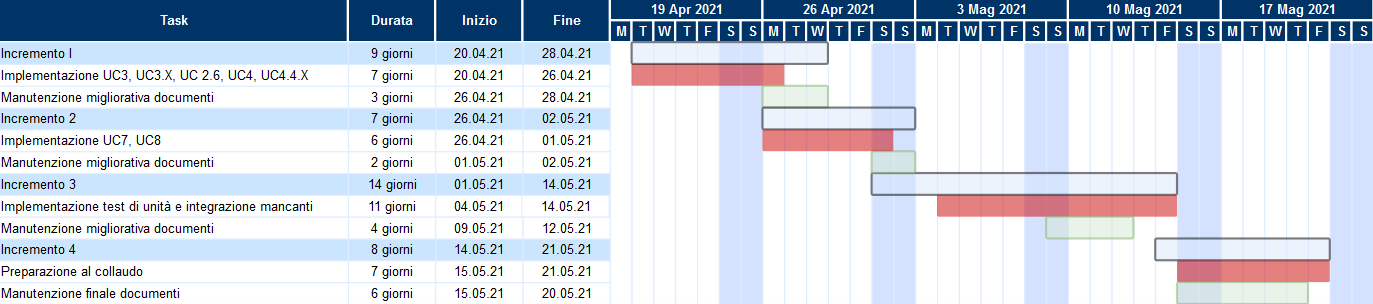
\includegraphics[width=\textwidth]{source/img/Validazione_collaudo.png}
        		\caption{Diagramma di Gantt dell'attività di validazione e collaudo}
    		\end{figure}
	\subsubsection{Tabella incrementi}
	\begin{longtabu} to \textwidth{| X[0.2, c m] | X[0.4, l m ] |}
		\hline
		\textbf{Nome} & \textbf{Descrizione} \\ 
	 \hline
		 \textbf{Incremento 1} & \textbf{Ore:} 50 \\
	 \hline
	 	Implementazione UC3, UC3.X, UC 2.6, UC4, UC4.4.X &
		Implementazione dei casi d'uso elencati. \\
	 \hline
		Manutenzione migliorativa dei documenti &
		In particolare: aggiornamento del Manuale Utente. \\
	 \hline
		 \textbf{Incremento 2} & \textbf{Ore:} 40 \\
	 \hline
	 	Implementazione UC7, UC8 &
		Implementazione dei casi d'uso elencati ed eventuali alti casi d'uso facoltativi. \\
	 \hline
		Manutenzione migliorativa dei documenti &
		In particolare: termine stesura del Manuale del Manutentore e del Manuale Utente. \\
	 \hline
	 	\textbf{Incremento 3} & \textbf{Ore:} 70 \\
	 \hline
		Implementazione test di unità e integrazione mancanti &
		Implementazione dei test con l'obiettivo di raggiungere la code coverage desiderata. \\
	 \hline
		 Manutenzione migliorativa documenti &
		 In particolare: eventuale aggiornamento del Piano di Qualifica per quanto riguarda i test di sistema e accettazione, correzione segnalazioni correzione RQ. \\
	 \hline
	 \textbf{Incremento 4} & \textbf{Ore:} 21\\
	 \hline
		 Preparazione al collaudo &
		 Preparazione del materiale necessario al collaudo, ultime verifiche al codice prodotto. \\
	 \hline
		 Manutenzione migliorativa documenti &
		 In particolare: stesura consultivo e analisi di periodo, offerta finale ed esposizione delle metriche raccolte. \\
	 \hline
 \end{longtabu}
 